\documentclass{article}
\usepackage{tabularx,fullpage,url}
\usepackage[top=1in, bottom=1in, left=.5in, right=.75in]{geometry}
\usepackage{amsmath,amssymb,graphicx,amsthm,xparse, color, mathrsfs} 
\usepackage{ epstopdf, fullpage}

\usepackage[ruled,vlined]{algorithm2e}
\usepackage{xifthen}
\usepackage{wrapfig}

\newcommand{\mypagebreak}{\begin{center}
		\noindent\makebox[\linewidth]{\rule{7.5in}{1pt}}
	\end{center}}
\bibliographystyle{siam}
\newcommand{\minimize}[1]{\underset{#1}{\text{minimize}}}
\newcommand{\maximize}[1]{\underset{#1}{\text{maximize}}}
\newcommand{\mini}[1]{\underset{#1}{\text{min}}}
\newcommand{\argmin}[1]{\underset{#1}{\text{argmin}}}
\newcommand{\st}{\text{subject to}}
\newcommand{\rank}{\textbf{rank}}
\newcommand{\epi}{\mathbf{epi}}

\newcommand{\diag}{\textbf{diag}}
\newcommand{\mb}{\mathbf}
\newcommand{\R}{\mathbb R}
\newcommand{\mle}{\mathbf{MLE}}
\newcommand{\map}{\mathbf{MAP}}
\newcommand{\bE}{\mathbb E}
\newcommand{\mL}{\mathcal L}
\newcommand{\mH}{\mathcal H}
\newcommand{\mB}{\mathcal B}
\newcommand{\mN}{\mathcal N}
\newcommand{\mD}{\mathcal D}
\newcommand{\mC}{\mathcal C}

\newcommand{\mS}{\mathcal S}
\newcommand{\tr}{\mathbf{tr}}
\newcommand{\mrm}{\mathrm}
\newcommand{\proj}{\mathbf{proj}}
\newcommand{\prox}{\mathbf{prox}}
\newcommand{\sign}{\mathbf{sign}}
\newcommand{\range}{\mathbf{range}}
\newcommand{\var}{\mathbf{var}}
\newcommand{\vnull}{\mathbf{null}}
\newcommand{\pr}{\mathbf{Pr}}
\newcommand{\find}{\mathbf{find}}
\newcommand{\argmax}[1]{\underset{#1}{\mathrm{argmax}}}
\newcommand{\subjto}{\mathrm{subject~to}}


\newcommand{\red}[1]{{\color{red}#1}}
\newcommand{\blue}[1]{{\color{blue}#1}}

\newcommand{\gray}[1]{\textcolor{lightgray}{#1}}



\newcommand{\idx}[1]{{\scriptsize [#1]}}


\newcommand{\showpoints}[1]{\textbf{(#1)}}

\begin{document}
{\Large\textbf{CSE 353: Homework  \hfill
Due Friday, October 7 }}


\mypagebreak


\begin{enumerate}

\item \emph{Machine learning fundamentals.} \showpoints{3 pts, 1 pt each} In the following scenarios, decide if the i.i.d. (independent, identically distributed) assumption is reasonable. Justify your answer.


\begin{tabular}[t]{lll}
\begin{minipage}{.7\linewidth}
\begin{enumerate}
\item I am trying to decide if a child has COVID or not. There are several features I am measuring: fever presence, runny nose, sluggish behavior, complaints of headache. Are these features independent of each other? identically distributed across the children (conditioned on presence of COVID and no other information)?


\item Assume that poor Johnny has chronic asthma, and little Debbie has just recovered from bronchitis. The rest of the children are healthy. I measure the lung capacity of each child. Is this measurement identically distributed across all the children? Is it independent, assuming that these conditions are all noncontagious?



\item I now look at three adults, Amber, Brenda, and Chloe. Amber and Brenda both have children in the same kindergarten class. Chloe also has a child, but hers is in a different class. Are their chances of getting COVID independent? Identically distributed?



\end{enumerate}
\end{minipage}
&$\;$&
\begin{minipage}{.3\linewidth}
\centering
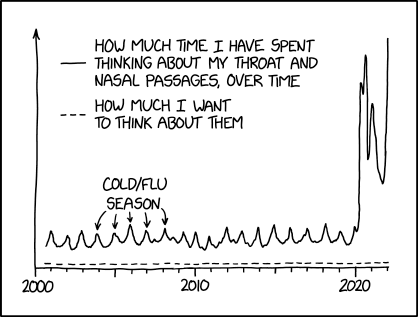
\includegraphics[width=\linewidth]{figs/throat_and_nasal_passages.png}\\(source: xkcd)
\end{minipage}
\end{tabular}


















\item \textbf{Entropy, conditional entropy, mutual information, information gain} \showpoints{2 pts}

I have a very messy sock drawer, containing 10 red socks, 5 blue socks, 4 yellow socks, and 1 black sock. 
\begin{enumerate}

\item \showpoints{0.5 pts} Recall the formula for entropy:
\[
H(X) = -\sum_{X=x} \pr(X=x)\log_2(\pr(X=x)). 
\]
Define $X$ a random variable which represents the color of a sock, randomly (uniformly) picked.  What is the entropy of this sock?


\item \showpoints{1 pt} My mom comes and tells me I must organize my socks better. So, I put all my red socks in the top drawer and the rest in my bottom drawer. Recall the formula for conditional entropy:
\[
H(X|Y) = -\sum_{X=x, Y=y} \pr(X=x,Y=y)\log_2(\pr(X=x|Y=y)). 
\]
What is the conditional entropy, where $X$ is the color of a sock randomly picked, and $Y$ is the drawer of which I pick it from? Assume that I pick the top drawer with twice the probability as picking the bottom drawer, but given a drawer, my choice of sock is uniformly distributed.



\item \showpoints{0.5 pts} The \emph{information gain} (also called \emph{mutual information}) can be defined in terms of the entropy and conditional entropy 
\[
I(X;Y) = H(X) - H(X|Y). 
\]
Give the mutual information between $X$ the color of the sock and $Y$ the drawer which it comes from. 




 
\end{enumerate}






\item \textbf{Decision trees.} \showpoints{2 pts}  In real life, you would use one of many highly optimized packages to program decision trees, but for the sake of understanding, here we will build a tiny decision tree on a simplified version of a multiclass classification problem, using our greedy method. 

\begin{itemize}
\item Download \texttt{covtype.zip},  which is a remote sensing classification problem (more details here \url{https://archive.ics.uci.edu/ml/datasets/covertype}). Inside there are two raw files: \texttt{covtype.info} and \texttt{covtype.data}. Skim \texttt{covtype.info} to understand the basic task. 

\item The file \texttt{covtype\_reduced.mat} has all the data already loaded and separated into a train and test set, and is subsampled severely to reduce computational complexity. (Like I said, this is a simple implementation. Go ahead and use scikit-learn for a ``full" version.)

\item The task is now to construct a decision tree classifier, that uses information gain to pick the best next split. Open the iPython notebook \texttt{covtype.ipynb}, and follow the instructions there.

\item Fill in the box to return functions that computes entropy and conditional entropy for a sequence of labels. Return the values given by the test problem provided in the notebook. Remember to include special cases for when one is required to take the log of 0. (We assume that $0\log_2(0) = 0$.)
To check your work, you should get:

\texttt{
entropy =  3.314182323161083, conditional entropy =  3.3029598816135173}


\item Fill in the box to return  a function that, at each step, given $X$, $y$, and a set of data sample indices to consider, returns the best feature to split and the best split value, as well as the indices split into two sets. (Follow the template in the iPython notebook). Again, return the solution to the test problem given.  Don't forget to handle the special case if the split results in an empty set--something special should happen, so the algorithm knows to reject this split.


\item The rest of the implementation is up to you. You can continue to use my iPython notebook, or you can implement your own decision tree using 1) your own implementation of trees and nodes, or 2) something you find online. What you \emph{cannot} do is to use an online implementation of a decision tree. (You can steal the tree, but not the decision part.) 


\item \textbf{My first step.} You can run the ``first step" box to start to debug your tree.
If you are using my implementation, if you have correctly filled in the holes and added the steps, you should get a result that looks similar to this. (The actual implementation of the split function can cause some variation.)

\begin{verbatim}
printing tree...
    root 0 2.0 leaf nodes  100 number of samples
current train err: 0.47
current test err: 0.5
printing tree...
    root 0 2.0 split 0, val 2930.62
    0 1 2.0 leaf nodes  41 number of samples
    0 2 1.0 leaf nodes  59 number of samples
one step train err: 0.41
one step test err: 0.42
\end{verbatim}

\item \showpoints{0.5 pt} Report your train and test misclassification rate for 25 steps of training. 


\item \showpoints{1 pt} Sketch out the resulting tree. (I recommend using a big piece of paper or a whiteboard + camera.) 


\item  \showpoints{0.5 pt}  Did your tree overfit? What are some hints that this may have happened?


\end{itemize}




























\item \emph{Hidden Markov Model spellchecker.} \showpoints{3 pts}
In this exercise we will make a spell-checker using a HMM. To do this, download \texttt{alice\_nlp\_release.ipynb} and follow the instructions.

\begin{itemize}
\item Read through the first two blocks to get an idea of what the task is. The idea is to go through the corrupted corpus, identify words which have probably been corrupted, and correct them probabilistically. 

\item In the 4th box, fill in the functions to construct the word probabilities (weighted frequencies in uncorrupted corpus) and transition matrix (which gives Pr(word $|$ prev word)). If done correctly, the lines printed out should read 

\begin{verbatim}
prob. of "alice" 0.014548615047424706
prob. of "queen" 0.002569625514869818
prob. of "chapter" 0.0009069266523069947
\end{verbatim}

with smoothing

\begin{verbatim}
prob. of "the alice" 0.00025406504065040653
prob. of "the queen" 0.016514227642276422
prob. of "the chapter" 0.012957317073170731
\end{verbatim}

no smoothing

\begin{verbatim}
prob. of "the alice" 0.0
prob. of "the queen" 0.03968253968253968
prob. of "the chapter" 0.0
prob. of "the hatter" 0.031135531135531136
\end{verbatim}

\item In the 5th box, fill in the function for computing the emission probability. The first 10 words closest to Alice should be 

\begin{verbatim}
['abide', 'alice', 'above', 'voice', 'alive', 'twice', 'thick', 'dance', 'stick', 'prize']
\end{verbatim}

\item Construct and run your Hidden Markov Model spell checker using the functions computed for the prior probabilities, emission probabilities, and transition probabilities. List some words whose spelling was corrected correctly, and some examples where the spell-correcter did not work as expected. Report the recovery rate of the ``fixed" corpus.




\end{itemize}



\end{enumerate}

\end{document}